% ============================================================
%  HITO 3 — Integracion Final, Escalabilidad y Validacion Integral
%  CleanPool App — Ingenieria de Software II
% ============================================================
\documentclass[11pt, a4paper]{article}

% ── Codificacion y lenguaje ──────────────────────────────────
\usepackage[utf8]{inputenc}
\usepackage[T1]{fontenc}
\usepackage[spanish, es-tabla]{babel}

% ── Tipografia ───────────────────────────────────────────────
\usepackage{lmodern}
\usepackage{microtype}

% ── Geometria ────────────────────────────────────────────────
\usepackage[top=2.5cm, bottom=2.5cm, left=3cm, right=3cm]{geometry}

% ── Color ────────────────────────────────────────────────────
\usepackage[table]{xcolor}
\definecolor{primary}{RGB}{31, 73, 125}
\definecolor{accent}{RGB}{192, 0, 0}
\definecolor{success}{RGB}{0, 112, 60}
\definecolor{rowgray}{RGB}{240, 243, 248}

% ── Tablas ───────────────────────────────────────────────────
\usepackage{tabularx}
\usepackage{booktabs}
\usepackage{array}
\usepackage{ltablex}
\usepackage{longtable}
\usepackage{textcomp}
\usepackage{amssymb}
\renewcommand{\arraystretch}{1.35}

% ── Listas ────────────────────────────────────────────────────
\usepackage{enumitem}
\setlist[itemize]{itemsep=3pt, topsep=4pt, leftmargin=1.6em}
\setlist[enumerate]{itemsep=3pt, topsep=4pt, leftmargin=1.8em}

% ── Secciones ────────────────────────────────────────────────
\usepackage{titlesec}
\titleformat{\section}
  {\large\bfseries\color{primary}}
  {\thesection.}{0.6em}{}
  [\vspace{-0.4em}\textcolor{primary}{\rule{\linewidth}{0.7pt}}\vspace{0.2em}]
\titleformat{\subsection}
  {\normalsize\bfseries\color{primary}}
  {\thesubsection.}{0.5em}{}
\titleformat{\subsubsection}
  {\normalsize\itshape\color{primary}}
  {}{0pt}{}

% ── Encabezado y pie ─────────────────────────────────────────
\usepackage{fancyhdr}
\pagestyle{fancy}
\fancyhf{}
\renewcommand{\headrulewidth}{0.4pt}
\fancyhead[L]{\small\color{gray} Hito 3 — Ingeniería de Software II}
\fancyhead[R]{\small\color{gray} \textit{Nombre del equipo}}
\fancyfoot[C]{\small\thepage}

% ── Hipervinculos ────────────────────────────────────────────
\usepackage[hidelinks]{hyperref}

% ── Espacio entre parrafos ───────────────────────────────────
\usepackage{parskip}
\setlength{\parskip}{6pt}

% ── Gráficos ─────────────────────────────────────────────────
\usepackage{graphicx}
\usepackage{float}

% Rutas de imagen (funciona tanto si compilas desde la raiz como desde ./hito3)
\graphicspath{{figuras/}{hito3/figuras/}}

% ============================================================
%  DATOS DEL EQUIPO (editar aqui)
% ============================================================
\newcommand{\nombreequipo}{Cleanpool}
\newcommand{\nombreproyecto}{CleanPool App}
\newcommand{\integrantes}{%
  Vicente Araya (PM) \quad|\quad
  Diego Carmona (SM) \quad|\quad
  Daniel Cortez \quad|\quad
  Constanza Malebran
}
\newcommand{\seccion}{300}
\newcommand{\fechaentrega}{20 de mayo de 2026}

% ============================================================
\begin{document}

% ============================================================
% ── Portada ──────────────────────────────────────────────────
% ============================================================
\thispagestyle{empty}
\begin{center}
  \vspace*{1.5cm}

  {\small\color{gray} Universidad Andres Bello \quad·\quad Ingenieria de Software II}

  \vspace{1cm}
  \textcolor{primary}{\rule{\linewidth}{1.5pt}}
  \vspace{0.4cm}

  {\Huge\bfseries\color{primary} Hito 3}\\[0.5em]
  {\LARGE Integracion Final, Escalabilidad y}\\
  {\LARGE Validacion Integral}

  \vspace{0.4cm}
  \textcolor{primary}{\rule{\linewidth}{1.5pt}}
  \vspace{1.2cm}

  {\Large\bfseries \nombreproyecto}

  \vspace{1cm}
  \begin{tabular}{rl}
    \textbf{Equipo:}      & \nombreequipo \\[4pt]
    \textbf{Seccion:}     & \seccion \\[4pt]
    \textbf{Entrega:}     & \fechaentrega \\[4pt]
    \textbf{Integrantes:} & \parbox[t]{9cm}{\integrantes}
  \end{tabular}

  \vfill
  {\small\color{gray} Documento de entrega oficial — semestre activo}
\end{center}

\newpage

% ============================================================
% ── Indice ───────────────────────────────────────────────────
% ============================================================
\tableofcontents
\newpage

% ============================================================
%  1. Estado General del Proyecto
% ============================================================
\section{Estado General del Proyecto}

\subsection{Resumen Ejecutivo}
El sistema \textbf{CleanPool App} integra monitoreo IoT para piscinas residenciales mediante sensores que publican lecturas (ej. temperatura y ORP) hacia un broker MQTT. El \textbf{frontend} (Flutter) consulta y visualiza el estado de las piscinas, mientras que el \textbf{backend} (FastAPI) expone endpoints protegidos (JWT) para la gestion de usuarios y piscinas.

En el contexto de Hito 3, el foco de integracion final se centra en: (i) consolidar el flujo completo desde la ingestion de datos IoT hasta la evaluacion del estado (priorizando sensor sobre mantencion manual) y (ii) asegurar que el despliegue sea repetible mediante contenedores Docker y automatizacion con GitHub Actions / Dokploy.

\subsection{Objetivos Alcanzados}
\textbf{Objetivo funcional:}
Se implementan y validan flujos de autenticacion JWT, CRUD de piscinas, calculo y persistencia de tratamientos manuales, registro historico de mantenciones y evaluacion de estado de piscina usando reglas que priorizan lecturas de sensores frescas sobre datos manuales.

\textbf{Objetivo tecnico:}
Se consolida una arquitectura de despliegue con \textbf{Docker Compose} (MongoDB, Mosquitto MQTT, backend FastAPI y frontend), y se integra un worker MQTT en segundo plano que suscribe y persiste lecturas en MongoDB. Adicionalmente, se incorporan \textbf{logs estructurados} persistidos en MongoDB para trazabilidad de requests.

\textbf{Objetivo de negocio:}
Se entrega una solucion operativa que reduce la dependencia de verificacion manual esporadica, permitiendo al usuario visualizar el estado de aptitud y mantener trazabilidad de mantenciones.

\subsection{Estado de Madurez del Sistema}
\begin{longtable}{@{} p{3cm} p{11.2cm} @{}}
  \toprule
  \textbf{Componente} & \textbf{Estado actual} \\
  \midrule
  Frontend & Operativo: app Flutter con consumo REST (login, CRUD de piscinas, estado y mantenciones). Evidencia visual incluida en el Anexo A. \\
  \midrule
  Backend & Operativo: FastAPI con endpoints para autenticacion, gestion de piscinas, lectura del estado (sensor > manual), mantenciones, tratamiento manual y ingestion IoT. \\
  \midrule
  Base de datos & Operativo: MongoDB en contenedor (persistencia de colecciones como \texttt{pools}, \texttt{mantenciones}, \texttt{lecturas} y \texttt{device\_bindings}). \\
  \midrule
  Integraciones & Operativo: Mosquitto MQTT (topics de sensores) con ingestion hacia MongoDB, utilizando API key para proteger la ingestion HTTP legacy. \\
  \midrule
  Infraestructura & Operativo: stack reproducible con Docker Compose y despliegue automatico (Dokploy y/o workflow de CI/SSH). \\
  \midrule
  Testing & Operativo: se ejecutan pruebas backend con \texttt{pytest} (y pruebas frontend con \texttt{flutter test} en CI). \\
  \bottomrule
\end{longtable}

% ============================================================
%  2. Arquitectura Final del Sistema
% ============================================================
\section{Arquitectura Final del Sistema}

\subsection{Arquitectura Integrada}
\begin{center}
\begin{tabular}{@{}l l@{}}
  \textbf{Frontend (Flutter)} & \textbf{Backend (FastAPI)} \\
  \\
  \scriptsize Consume endpoints REST: \texttt{/auth/\ldots}, \texttt{/piscinas/\ldots}, \texttt{/mantenciones/\ldots}, \texttt{/piscinas/\{id\}/status}. & \scriptsize Exposicion y validacion de endpoints; procesamiento de reglas; worker MQTT y logs. \\
  \\
  \textbf{MongoDB (Atlas / contenedor)} & \textbf{Mosquitto MQTT} \\
  \\
  \scriptsize Persistencia: piscinas, mantenciones, lecturas y historial/logs. & \scriptsize Broker para lecturas IoT (topics por dispositivo/piscina). \\
\end{tabular}
\end{center}

\vspace{0.5em}
\noindent\textbf{Flujo principal:} Sensor IoT publica hacia Mosquitto $\rightarrow$ worker MQTT persiste lecturas en MongoDB $\rightarrow$ backend evalua estado (sensor frescos > manual) $\rightarrow$ frontend muestra estado y recomendaciones.

\subsection{Integracion de Componentes}
\begin{longtable}{@{} p{2.6cm} p{5.4cm} p{5.1cm} @{}}
  \toprule
  \textbf{Componente} & \textbf{Integracion realizada} & \textbf{Resultado} \\
  \midrule
  Frontend (Flutter) & Consumo de APIs REST, gestion de sesion JWT y visualizacion del estado de piscina. & Operativo (ver Anexo A). \\
  \midrule
  Backend (FastAPI) & Endpoints para auth, CRUD de piscinas, status unificado (sensor > manual) y mantenciones; worker MQTT en segundo plano. & Operativo. \\
  \midrule
  Base de datos (MongoDB) & Persistencia de colecciones operativas (\texttt{pools}, \texttt{mantenciones}, \texttt{lecturas}, \texttt{device\_bindings}) y logs estructurados. & Operativo. \\
  \midrule
  APIs / ingestion IoT & Ingestion MQTT (worker) y endpoints legacy protegidos (API key). & Parcial/operativo segun via (MQTT y REST). \\
  \bottomrule
\end{longtable}

\subsection{Escalabilidad y Rendimiento}
\begin{longtable}{@{} p{2.5cm} p{6.3cm} p{5.4cm} @{}}
  \toprule
  \textbf{Aspecto} & \textbf{Implementacion} & \textbf{Impacto esperado} \\
  \midrule
  Contenedores & Docker Compose separa servicios (MongoDB, Mosquitto, backend, frontend). & Facil despliegue y escalamiento horizontal por servicio. \\
  \midrule
  Ingestion IoT & Worker MQTT ejecuta en hilo en background y persiste lecturas en MongoDB. & Reduccion de latencia percibida en endpoints REST. \\
  \midrule
  Evaluacion sensor vs manual & Regla \texttt{is\_reading\_fresh} utiliza ventana de frescura (2 minutos) para decidir fuente confiable. & Evita resultados obsoletos y mejora estabilidad del estado. \\
  \midrule
  Logs y trazabilidad & Middleware mide latencia request y persiste logs estructurados en MongoDB. & Mejora monitoreo y debugging para mantener calidad operativa. \\
  \bottomrule
\end{longtable}

% ============================================================
%  3. Validacion Funcional y Tecnica
% ============================================================
\section{Validacion Funcional y Tecnica}

\subsection{Funcionalidades Finales Implementadas}
\begin{longtable}{@{} p{1cm} p{4.2cm} p{9cm} p{2cm} @{}}
  \toprule
  \textbf{ID} & \textbf{Historia de usuario} & \textbf{Descripcion} & \textbf{Estado} \\
  \midrule
  HU-01 & Auth & Registro/login y acceso autenticado (JWT) y datos del usuario via \texttt{/auth/me}. & Completa \\
  \midrule
  HU-02 & Gestion de piscinas & CRUD de piscinas y consulta de estado de piscina (\texttt{/piscinas/\{id\}/status}), aplicando priorizacion sensor > manual. & Completa \\
  \midrule
  HU-03 & Ingestion IoT y mantencion & Ingestion de lecturas IoT (MQTT) y consolidacion de mantenciones/tratamientos con historial. & Completa \\
  \midrule
  HU-04 & Mantenciones & Registro y consulta del historial de mantenciones (\texttt{/mantenciones/}) y persistencia. & Completa \\
  \bottomrule
\end{longtable}

\subsection{Casos de Uso Validados}
Se validaron los siguientes casos de uso en el flujo principal del sistema:
\begin{itemize}
  \item El usuario autentica via JWT, obtiene su perfil (\texttt{/auth/me}) y gestiona sus piscinas (\texttt{/piscinas}).
  \item El usuario consulta el estado de una piscina con \texttt{/piscinas/\{id\}/status}. Cuando existen lecturas de sensor dentro de la ventana de frescura, el estado utiliza esos valores; si no, se apoya en mantencion manual mas reciente.
  \item Se registra mantencion manual (\texttt{/piscinas/\{id\}/tratamiento}) y se revisa historial (\texttt{/mantenciones/}).
  \item Se valida la ingestion IoT mediante MQTT: el backend suscribe los topics configurados y persiste lecturas en MongoDB, afectando el estado posterior.
\end{itemize}

\subsection{Pruebas Realizadas}
\begin{longtable}{@{} p{1cm} p{2.8cm} p{10.3cm} p{2cm} @{}}
  \toprule
  \textbf{ID} & \textbf{Tipo} & \textbf{Descripcion} & \textbf{Resultado} \\
  \midrule
  TP-01 & Unitaria & Validacion de servicios (ej. calculadora de aptitud, parser/validaciones) mediante \texttt{pytest}. & Pasa \\
  \midrule
  TP-02 & Integracion & Flujo end-to-end de integracion backend (auth, CRUD piscinas, status, mantenciones) con mocks y/o DB simulada. & Pasa \\
  \midrule
  TP-03 & E2E & Ejecucion manual guiada por swagger/curl segun \texttt{MANUAL\_DE\_PRUEBAS.md} para verificar retornos esperados. & Pasa \\
  \midrule
  TP-04 & Carga & Observacion de comportamiento bajo re-injection de redeploy (sin pruebas de carga automatizadas). & Observado \\
  \bottomrule
\end{longtable}

\subsection{Cobertura y Calidad}
Los tests backend se ejecutan en CI con \texttt{pytest tests/} y se ejecutan pruebas frontend con \texttt{flutter test}. En este proyecto, no se reporta un porcentaje de cobertura mediante \texttt{pytest-cov} en el workflow, por lo que la cobertura se evalua principalmente por el estado de ejecucion de pruebas y la calidad de casos cubiertos.

% ============================================================
%  4. Despliegue y Operación
% ============================================================
\section{Despliegue y Operacion}

\subsection{Infraestructura de Produccion}
\begin{longtable}{@{} p{3cm} p{11cm} @{}}
  \toprule
  \textbf{Elemento} & \textbf{Detalle} \\
  \midrule
  Plataforma & Servidor universitario (stack desplegado con Docker Compose; Dokploy para auto-deploy en rama \texttt{main}). \\
  \midrule
  Base de datos & MongoDB (contenedor Docker; persistencia via volumen \texttt{mongo\_data}). \\
  \midrule
  Contenedores & Docker Compose: servicios \texttt{mongo}, \texttt{mosquitto}, \texttt{backend}, \texttt{frontend}. \\
  \midrule
  CI/CD & GitHub Actions (tests) + Dokploy (auto-deploy via webhook) y/o despliegue por SSH con \texttt{docker compose up -d --build}. \\
  \midrule
  Dominio & \texttt{http://200.27.101.243} (Frontend: puerto 8884; API: puerto 8883; MongoDB: puerto 8885; MQTT: puerto 1883). \\
  \bottomrule
\end{longtable}

\subsection{Proceso de Despliegue}
El flujo de despliegue se basa en:
\begin{itemize}
  \item \textbf{CI:} cada push a \texttt{main} ejecuta \texttt{pytest} (backend) y \texttt{flutter test} (frontend).
  \item \textbf{Deploy:} Dokploy se configura para consumir \texttt{docker-compose.yml} y reconstruiar el stack, levantando los servicios en el servidor.
  \item \textbf{Alternativa por emergencia:} acceso SSH al servidor y ejecucion de \texttt{docker compose up -d --build}.
\end{itemize}

\subsection{Monitoreo y Logs}
El backend incorpora middleware que:
\begin{itemize}
  \item asigna un \texttt{request\_id},
  \item mide latencia por request,
  \item persiste \textbf{logs estructurados} en MongoDB (coleccion de logs) tanto para operaciones exitosas como excepciones no controladas.
\end{itemize}
Los logs se almacenan en BD de logs con base \texttt{cleanpool\_logs} y coleccion \texttt{api\_request\_logs}. Esto permite revisar el comportamiento del sistema y detectar errores o tiempos de respuesta anomales.

% ============================================================
%  5. Gestion Scrum y Trabajo Colaborativo
% ============================================================
\section{Gestion Scrum y Trabajo Colaborativo}

\subsection{Estado Final del Sprint}
Sprint evaluado: \textbf{Sprint 4} (Integracion final del sistema). En esta entrega se consolidan historias asociadas a autenticacion, gestion de piscinas, ingestion IoT, evaluacion de estado y mantenciones.

Objetivo principal: Integrar completamente el flujo sensor $\rightarrow$ evaluacion $\rightarrow$ estado en la aplicacion, asegurando un despliegue estable y repetible.

Historias completadas: \textbf{4} (HU-01 a HU-04). Historias pendientes: \textbf{0} para el alcance de Hito 3.
\linebreak
Resultado general: \textbf{aprobado para entrega} (segun ejecucion de pruebas CI y validaciones funcionales guiadas).

\subsection{Commits y Participacion}
\begin{longtable}{@{} p{4cm} p{10.5cm} p{2cm} @{}}
  \toprule
  \textbf{Integrante} & \textbf{Aporte principal} & \textbf{Commits (recientes)} \\
  \midrule
  Vicente Araya (PM) & Integracion backend-frontend, soporte a despliegue (Dokploy) y mejoras en la ingestion/evaluacion. & 30 \\
  \midrule
  Diego Carmona (SM) & Implementacion y mejoras de interfaz/funcionalidades en el frontend e integraciones asociadas. & 5 \\
  \midrule
  Daniel Cortez & Ajustes y mejoras especificas en features de frontend asociadas al sprint. & 5 \\
  \midrule
  Constanza Malebran & Refinamientos UI y contenido de pantallas (perfil/historial) durante sprint 4. & 3 \\
  \bottomrule
\end{longtable}

\subsection{Problemas y Resoluciones}
Problema: conflictos al redeploy (contenedores con nombre ya en uso) y/o permisos en Docker al ejecutar operaciones desde Dokploy.

Resolucion: se unifico el flujo de despliegue para usar un script previo de paro/kill del stack y se documentaron comandos SSH de emergencia (segun \texttt{deploy/DOKPLOY.md}) para asegurar reproducibilidad.

Problema: inconsistencias en la evaluacion del estado cuando no existen lecturas MQTT recientes.

Resolucion: se centralizo la logica con una ventana de frescura de \textbf{2 minutos} para decidir si el sensor esta ONLINE o si se utiliza mantencion manual mas reciente.

% ============================================================
%  6. Demostracion de Valor
% ============================================================
\section{Demostracion de Valor}

\subsection{Valor Entregado al Usuario}
El usuario recibe un estado de piscina con base en informacion mas confiable (sensor dentro de ventana) y un respaldo con mantencion manual cuando el sensor no presenta datos recientes. Esto habilita decisiones de mantenimiento mas consistentes y reduce la dependencia de chequeos manuales aislados.

\subsection{Evidencia Funcional}
Se adjuntan capturas del funcionamiento del sistema: autenticacion, gestion de piscinas, consulta de estado y secciones relacionadas con mantenciones/perfil (ver Anexo A).
\begin{itemize}
  \item Evidencia de flujo funcional en la aplicacion.
  \item Confirmacion visual de actualizaciones en estado y vistas del usuario.
\end{itemize}

\subsection{Retroalimentacion Obtenida}
La validacion realizada por el equipo y a traves del manual de pruebas indica que los endpoints y el comportamiento esperado se cumplen (registro/login, CRUD, status y mantenciones). Se recomienda continuar optimizando la experiencia de usuario (refinamiento visual) y ampliar evidencia de pruebas de carga automatizadas en futuros hitos.

% ============================================================
%  7. Conclusiones y Proximos Pasos
% ============================================================
\section{Conclusiones y Proximos Pasos}

\subsection{Conclusiones Tecnicas}
Se consolido una arquitectura integrada con ingestion IoT, persistencia en MongoDB, evaluacion de estado sensor > manual y despliegue reproducible con Docker Compose. La incorporacion de logs estructurados aporta trazabilidad para operacion y soporte.

\subsection{Aprendizajes del Equipo}
Se aprendio a mantener consistencia entre rutas oficiales y legacy, a formalizar validaciones por ventana temporal (online/stale) y a documentar el flujo de despliegue para evitar fallas por colisiones de contenedores.

\subsection{Trabajo Futuro}
1. Incorporar pruebas de carga automatizadas y monitoreo mas granular (p. ej., dashboards).
2. Mejorar cache/optimizar consultas criticas (si aplica) para reducir latencia en lecturas frecuentes.
3. Ampliar el soporte de evidencias (capturas y casos) para demos y evaluaciones futuras.

% ============================================================
%  Anexos
% ============================================================
\newpage
\appendix

\section{Capturas del Sistema}
\begin{figure}[H]
  \centering
  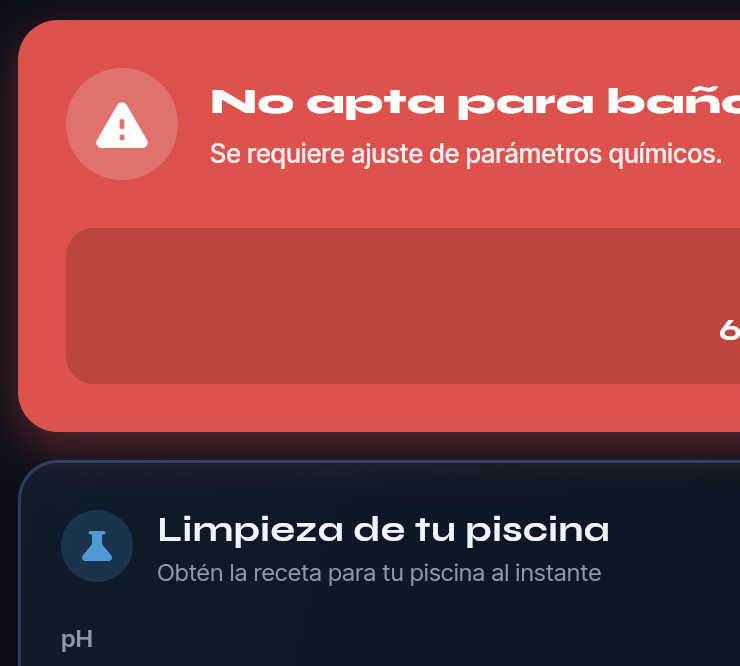
\includegraphics[width=0.95\linewidth]{captura_evidencia_func_01.png}
  \caption{Evidencia de flujo funcional 01}
\end{figure}
\vspace{0.5em}
\begin{figure}[H]
  \centering
  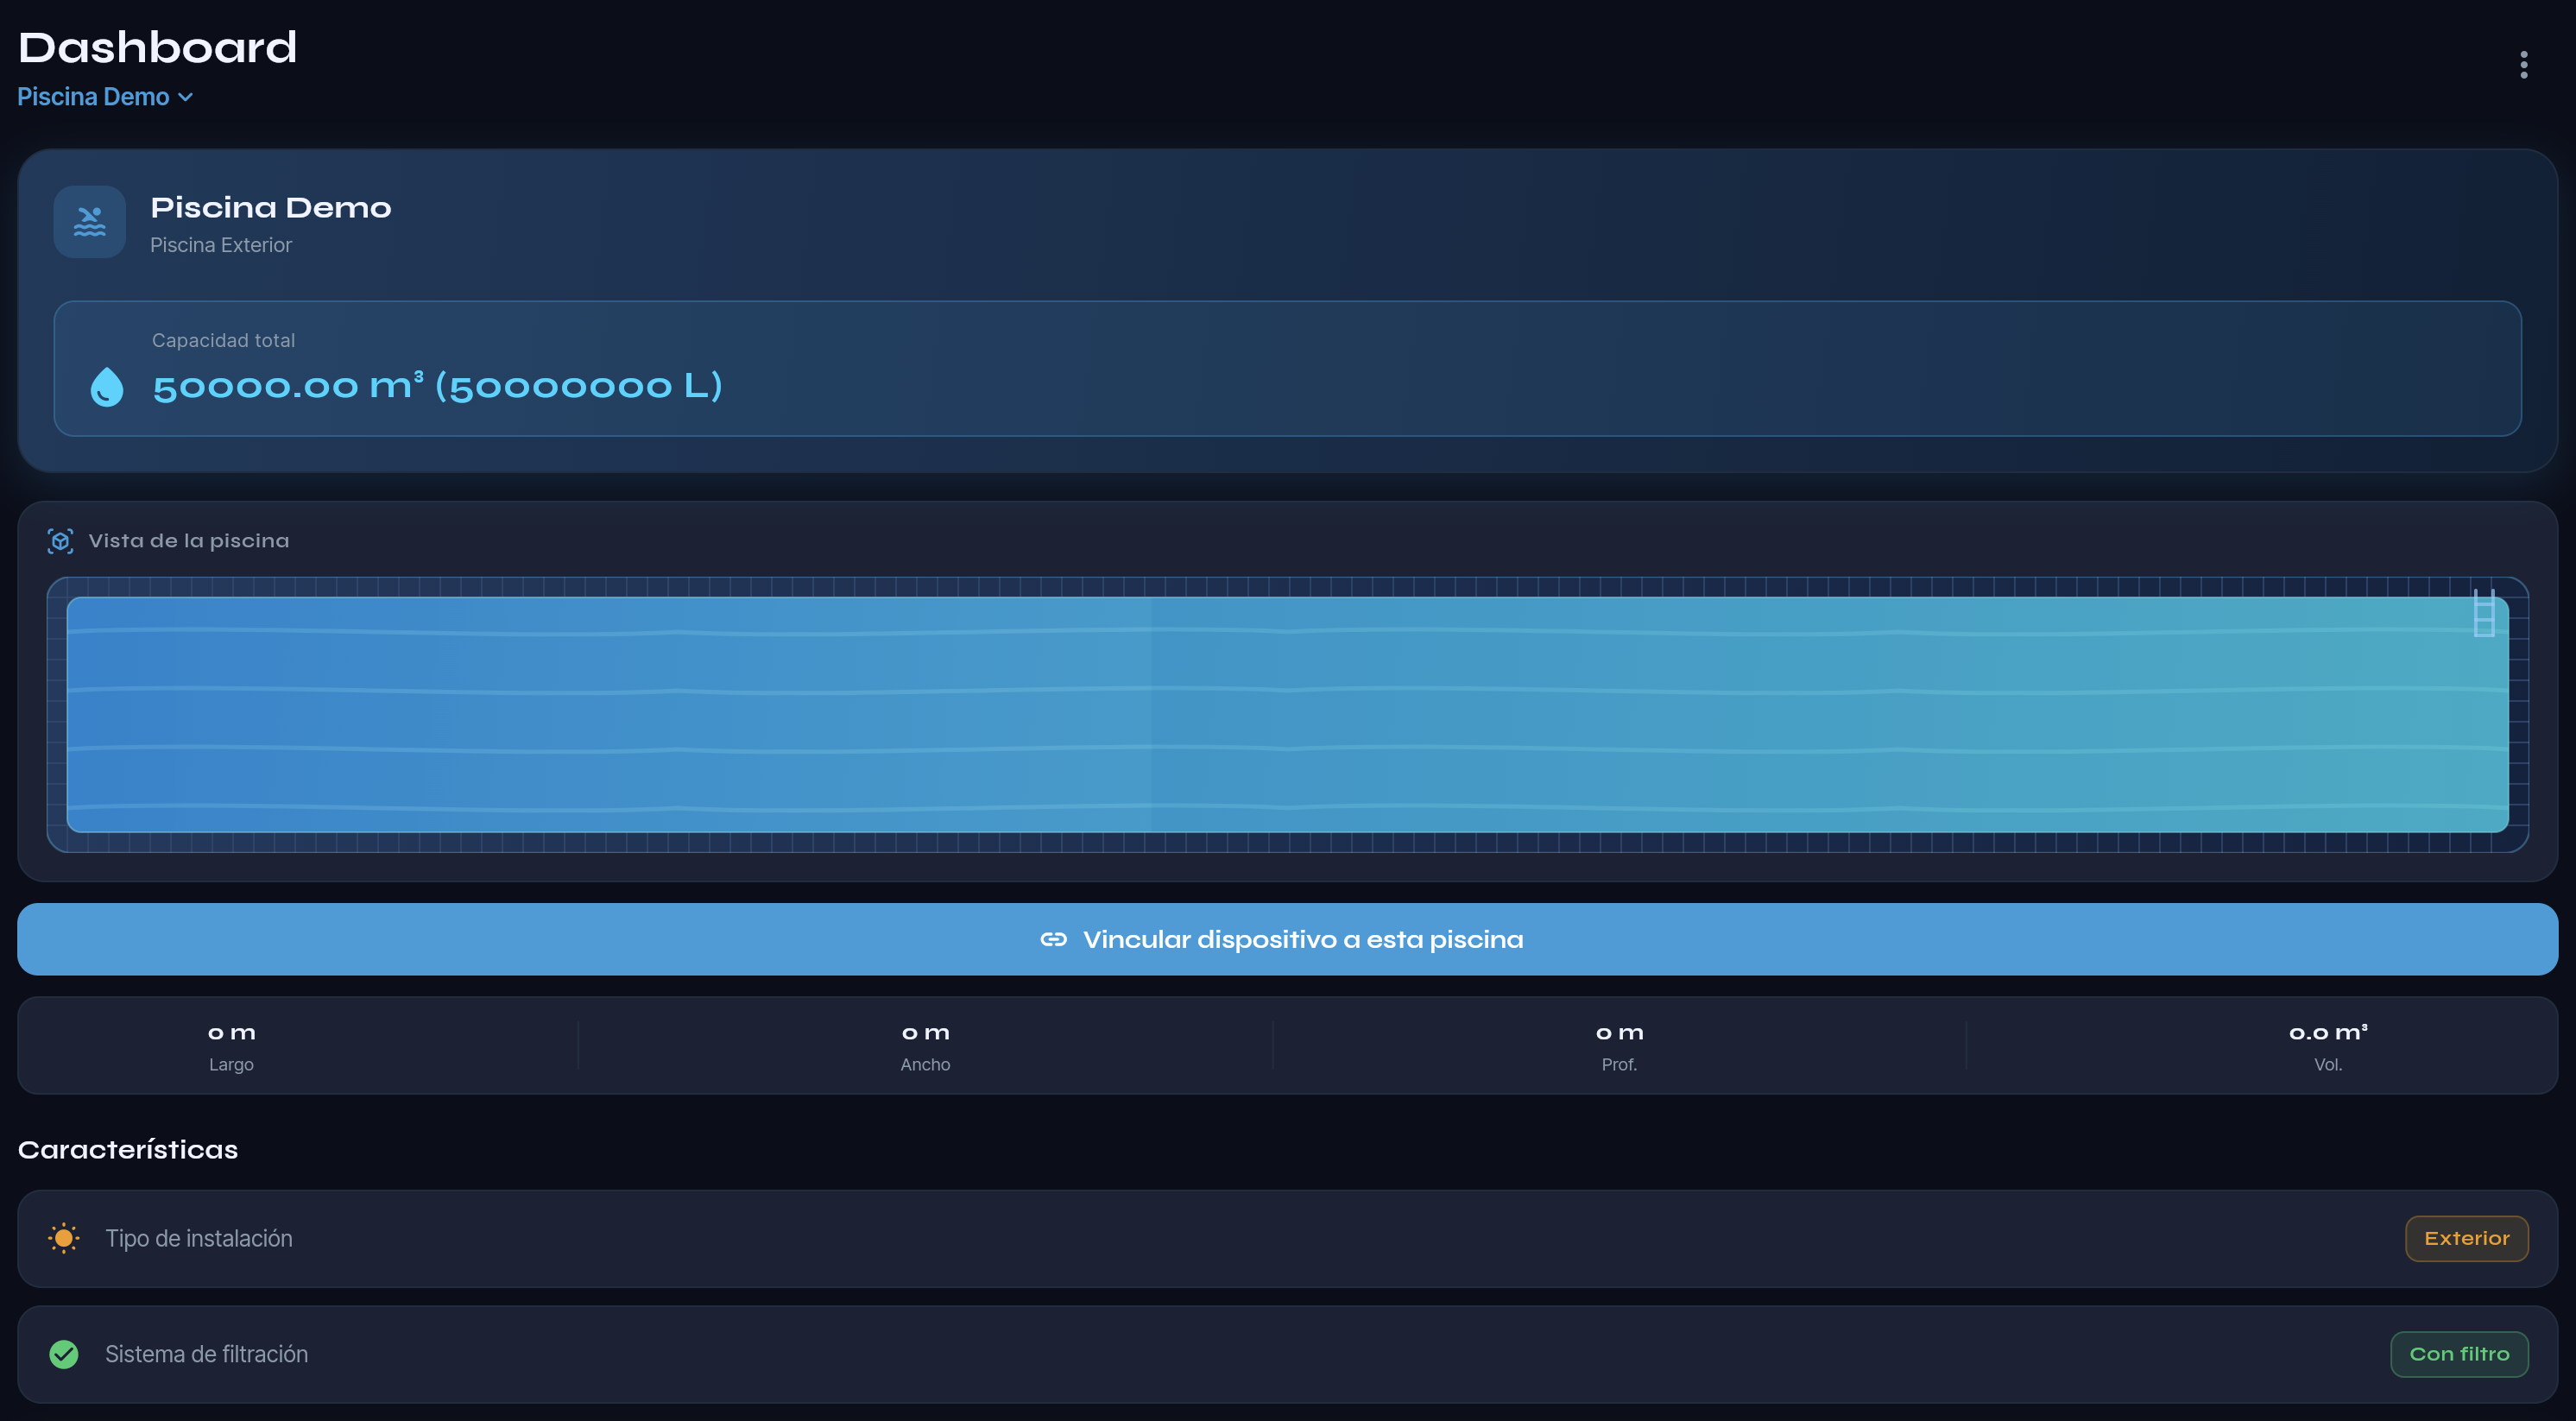
\includegraphics[width=0.95\linewidth]{captura_evidencia_func_02.png}
  \caption{Evidencia de flujo funcional 02}
\end{figure}
\vspace{0.5em}
\begin{figure}[H]
  \centering
  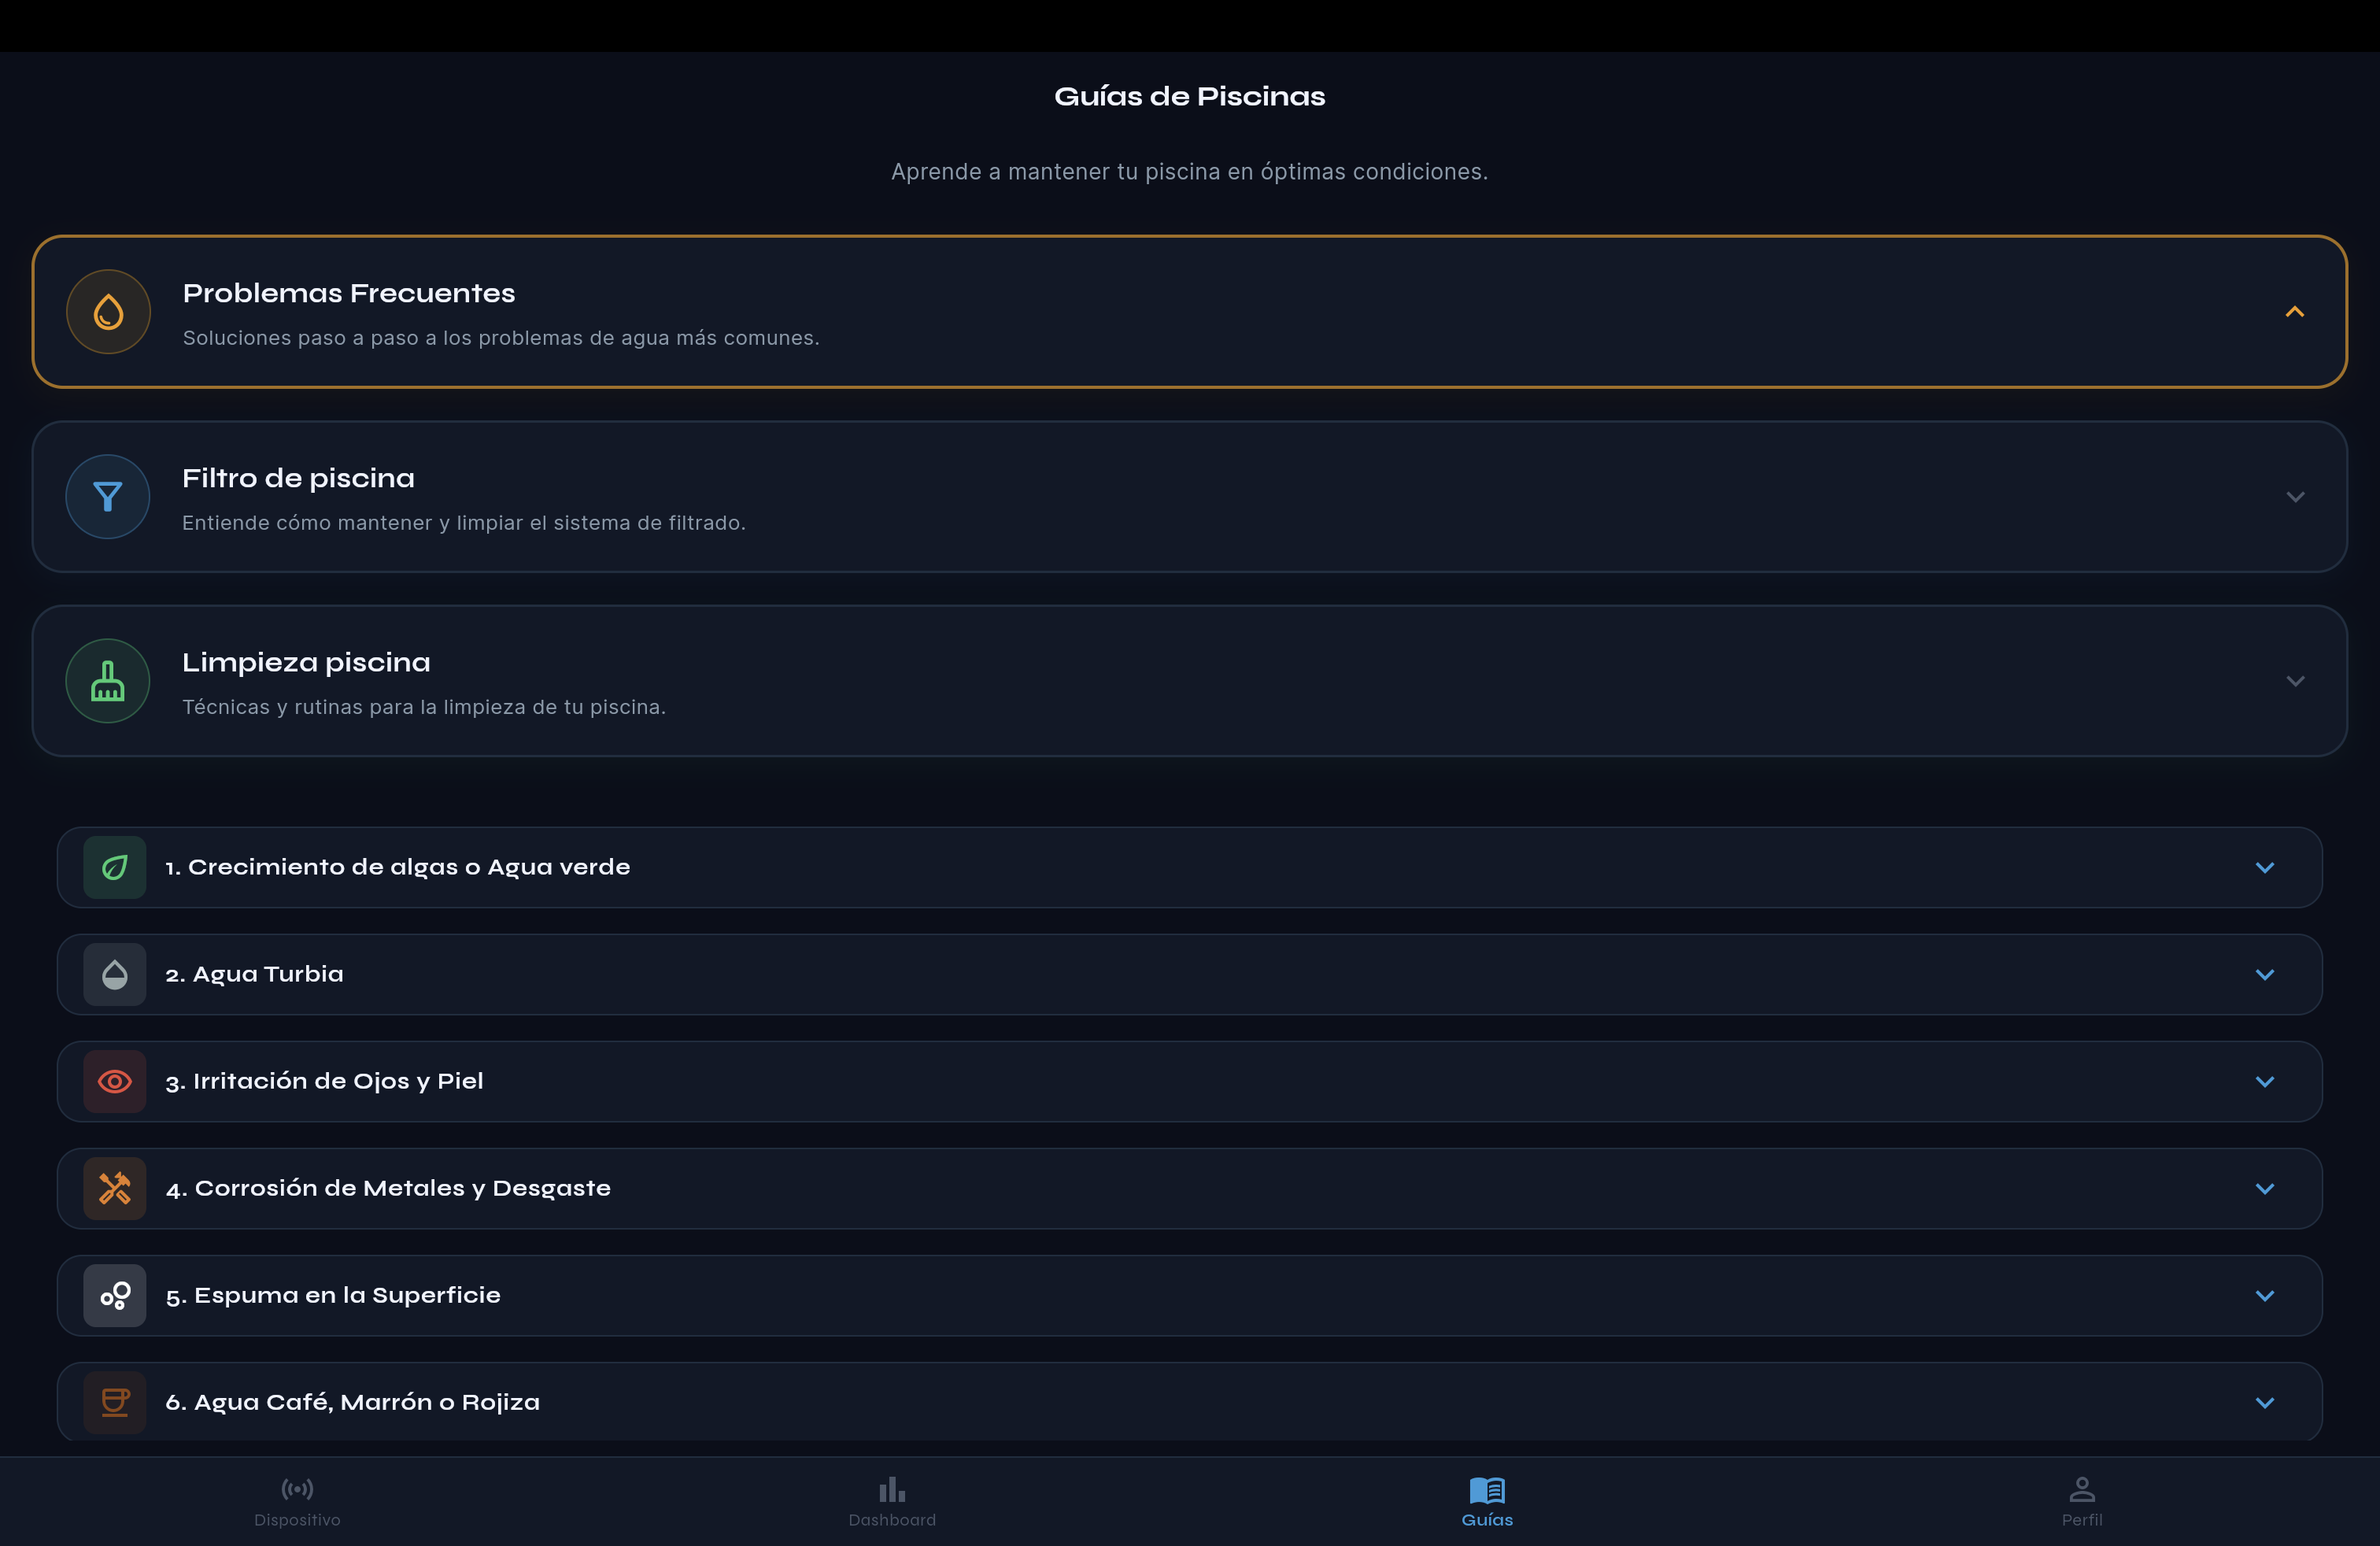
\includegraphics[width=0.95\linewidth]{captura_evidencia_func_03.png}
  \caption{Evidencia de flujo funcional 03}
\end{figure}
\vspace{0.5em}
\begin{figure}[H]
  \centering
  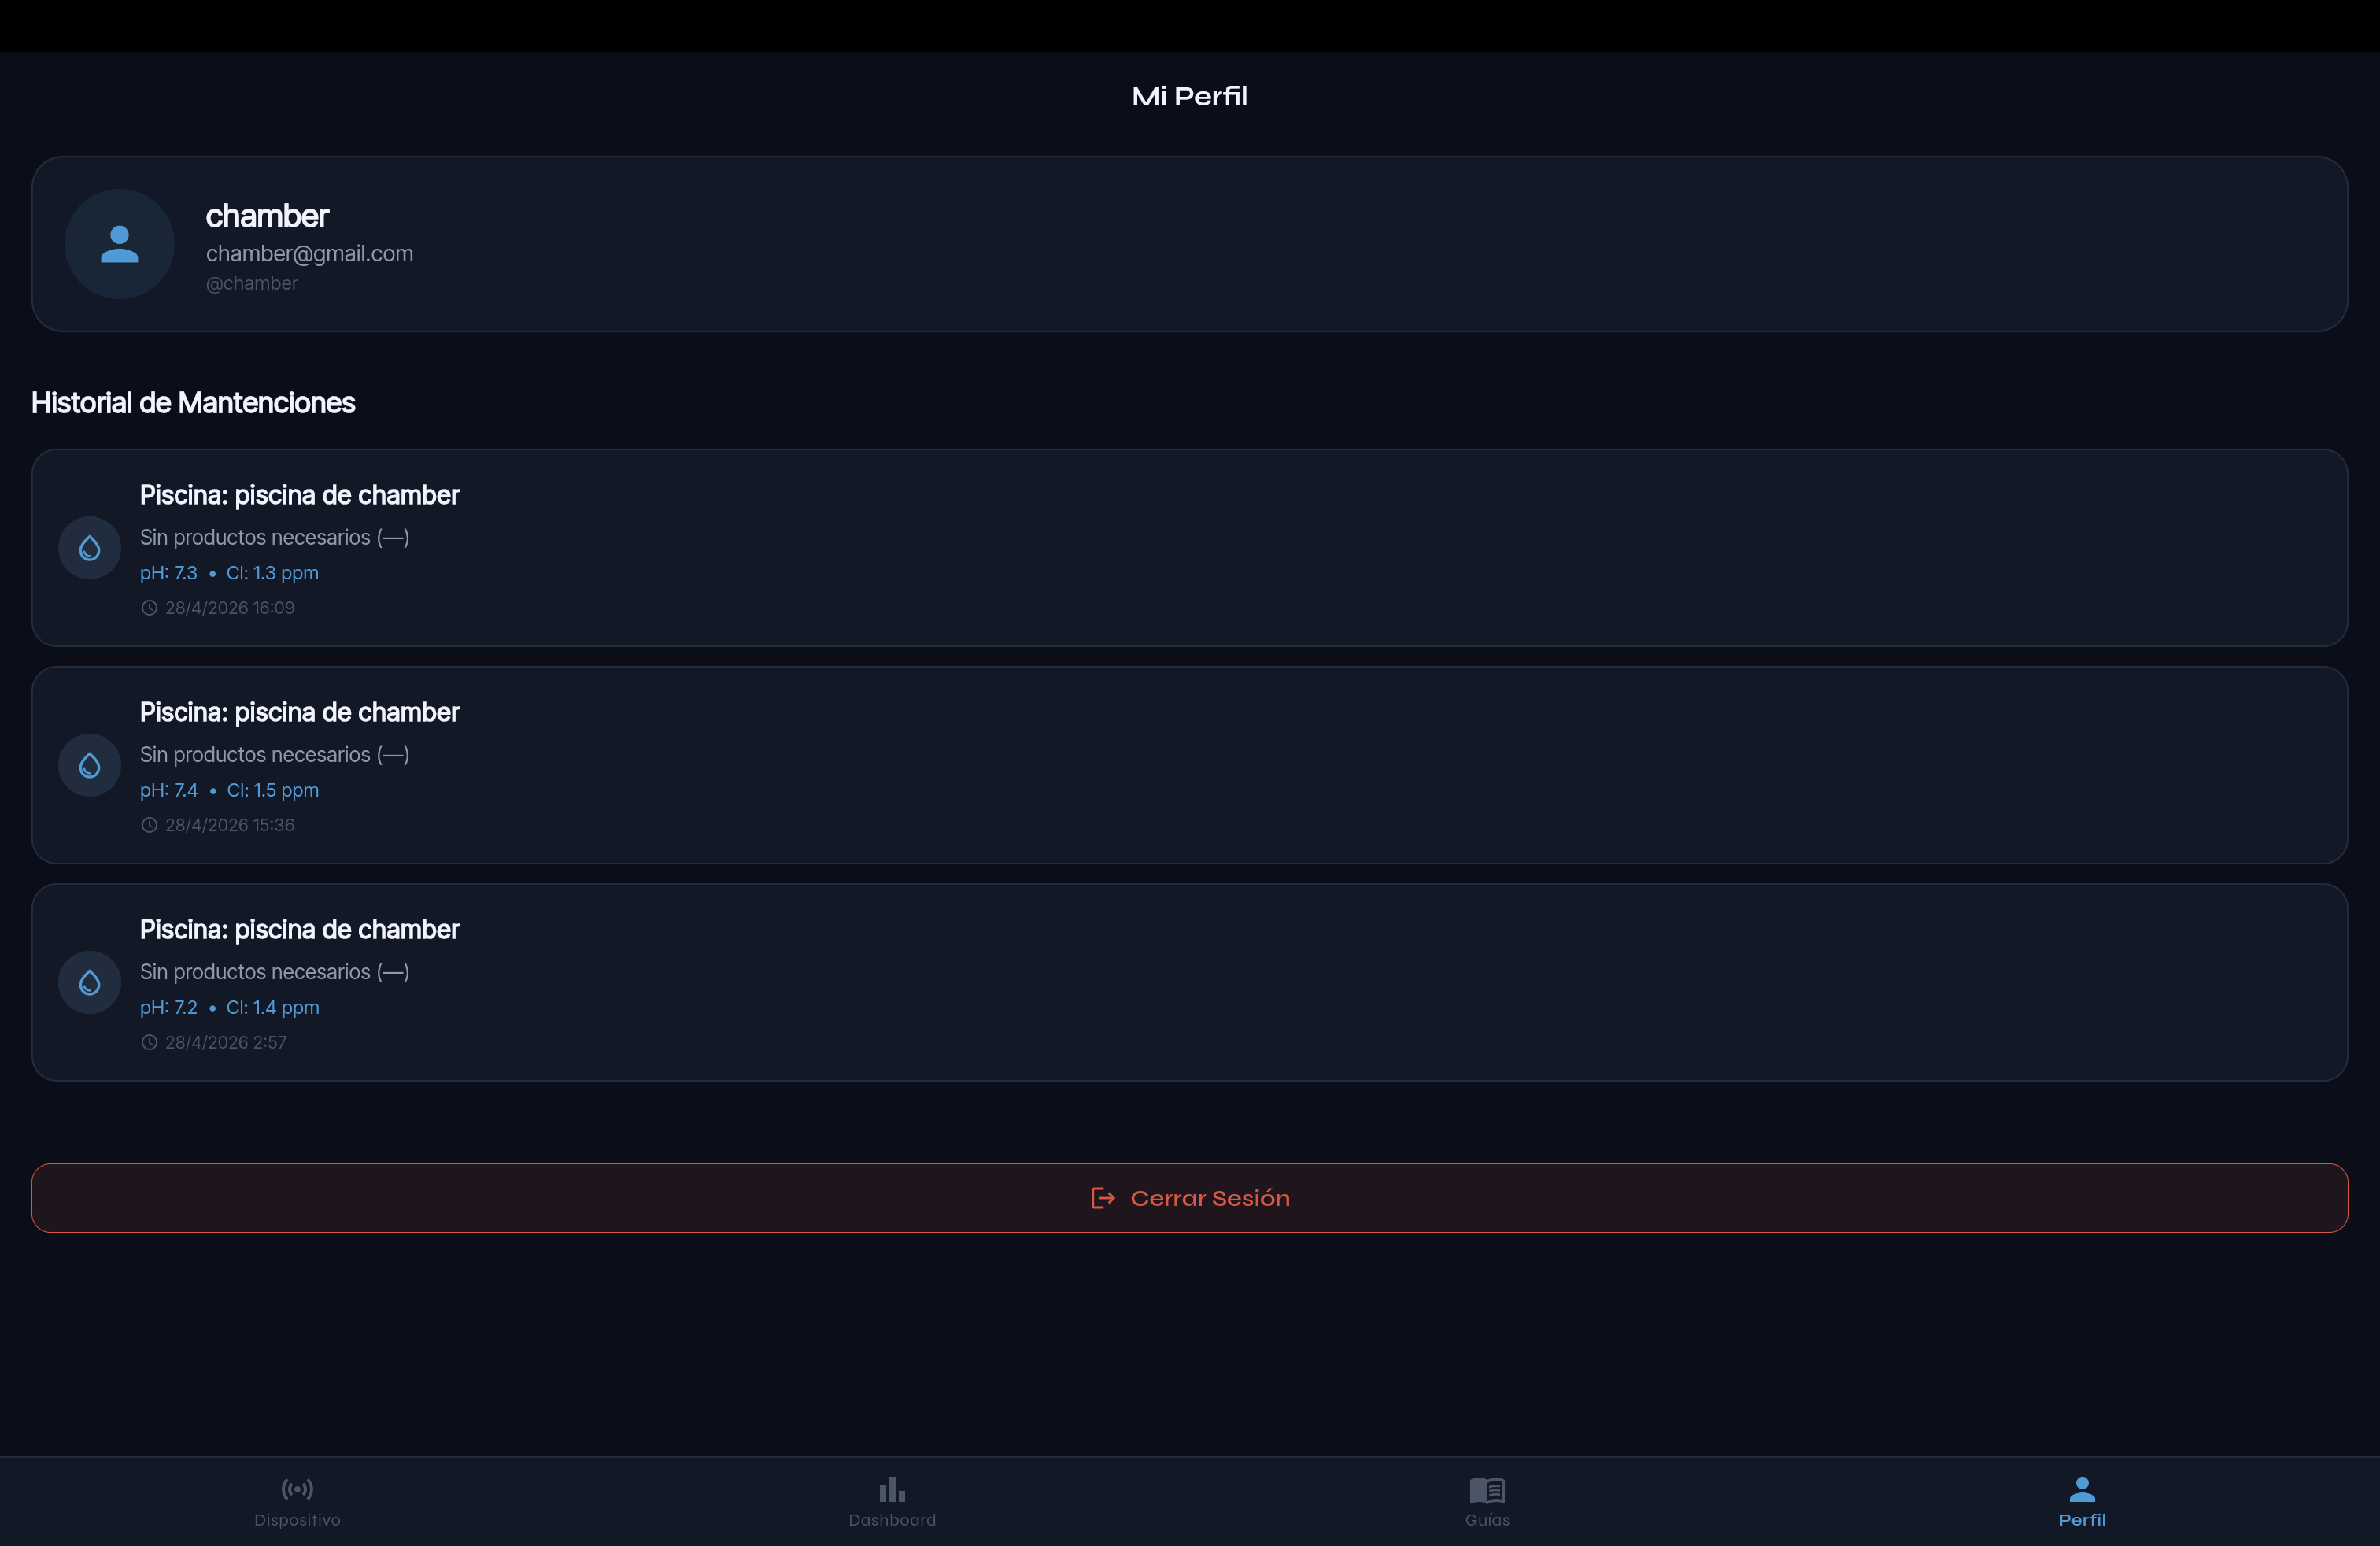
\includegraphics[width=0.95\linewidth]{captura_evidencia_func_04.png}
  \caption{Evidencia de flujo funcional 04}
\end{figure}
\vspace{0.5em}
\begin{figure}[H]
  \centering
  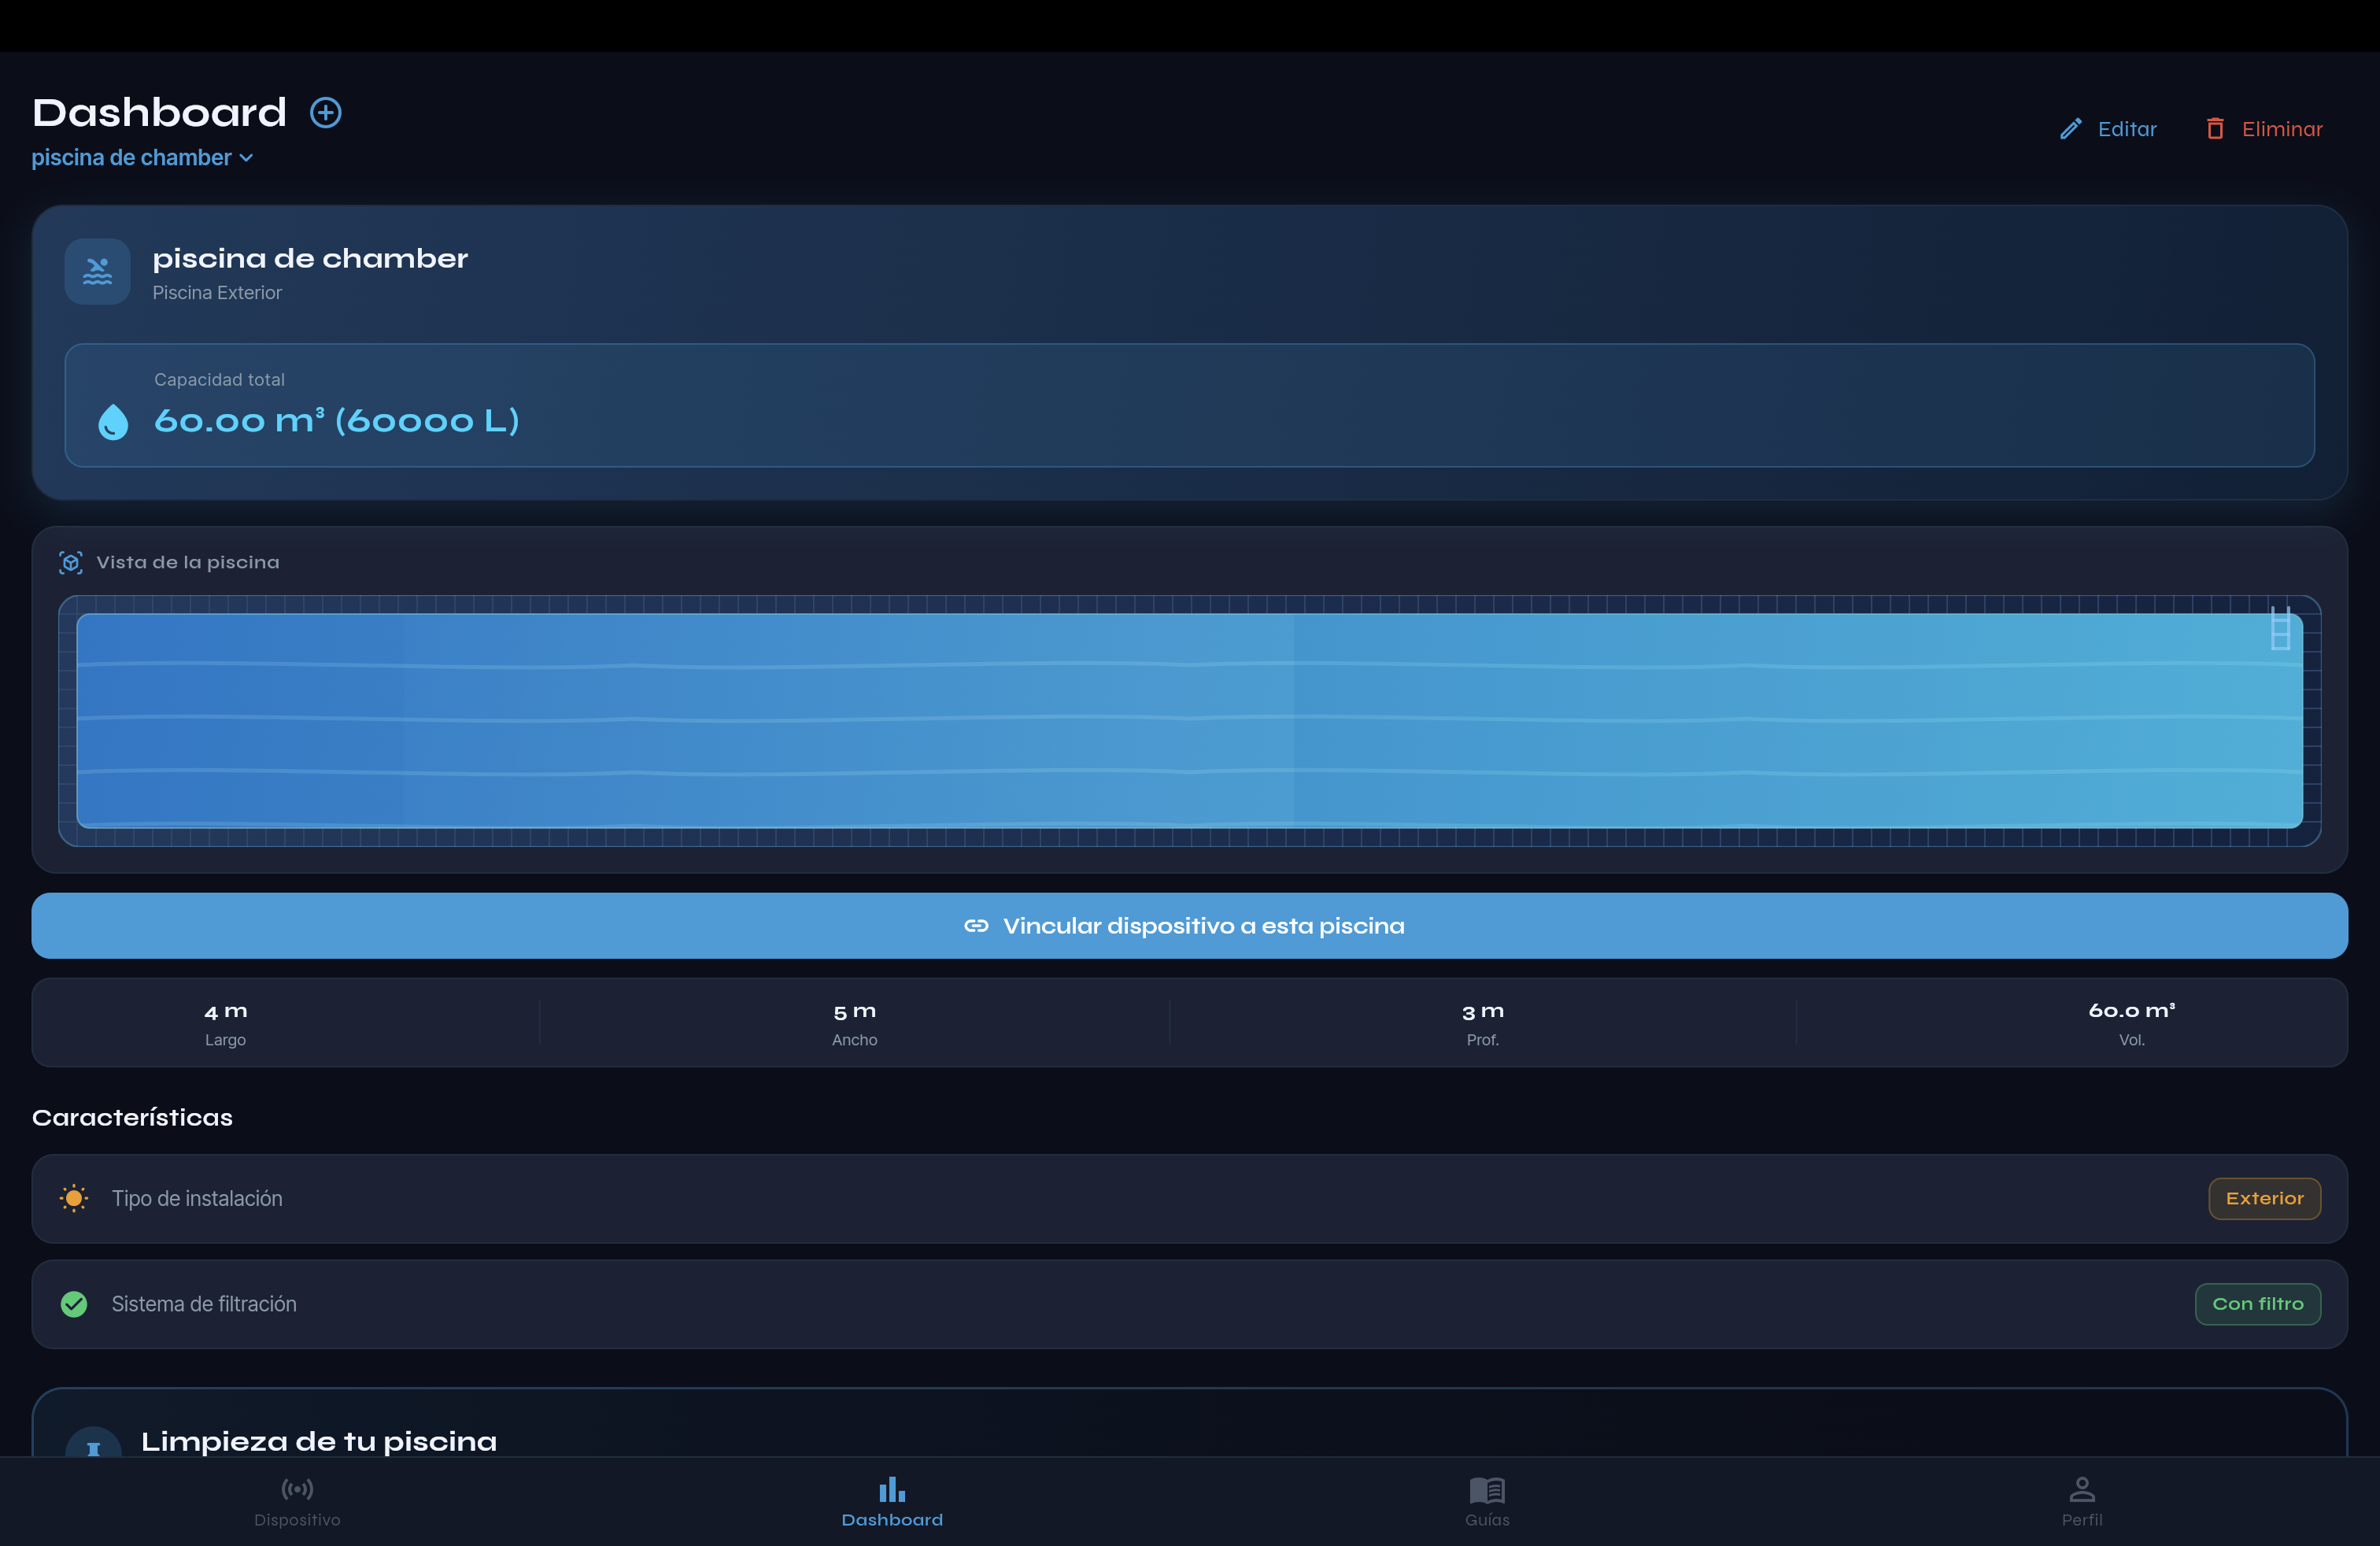
\includegraphics[width=0.95\linewidth]{captura_evidencia_func_05.png}
  \caption{Evidencia de flujo funcional 05}
\end{figure}

\section{Repositorio y Evidencias}
\begin{tabular}{@{} p{3.5cm} p{10.5cm} @{}}
  \toprule
  \textbf{Recurso} & \textbf{URL} \\
  \midrule
  Repositorio & \href{https://github.com/vicentearaya/software2}{https://github.com/vicentearaya/software2} \\
  Jira/Trello & (Pendiente / no utilizado en esta entrega) \\
  Produccion & \href{http://200.27.101.243:8884}{http://200.27.101.243:8884} \\
  \bottomrule
\end{tabular}

\section{Commits Relevantes}
\begin{enumerate}
  \item \texttt{3a7b99c}: lecturas sensor orp en app
  \item \texttt{88fb2fc}: cambio inicio
  \item \texttt{294b060}: botones para volver a inicio y al cerrar sesion volver inicio
  \item \texttt{48990e2}: prueba de redeploy sin eliminar contenedores
  \item \texttt{79c9b05}: prueba deploy
  \item \texttt{e6604fe}: probando redeploy
  \item \texttt{28c33f9}: docs: prueba autodeploy
  \item \texttt{9c5ceda}: fixes para autodeploy con dokploy
\end{enumerate}

\end{document}

